%!TEX root = ../memoire.tex

\chapter{Adaptation de GenDR}\label{ch:implementation}

Au chapitre précédent, nous avons expliqué comment nous avons extrait les informations de VerbNet à l'aide de scripts Python pour nous en servir dans GenDR. Ce chapitre couvrira l'adaptation de GenDR pour lui faire exploiter ces nouvelles données. D'abord, nous expliquerons comment nos dictionnaires fonctionnent après l'importation de VerbNet et comment ils communiquent entre eux. Puis, nous allons montrer comment fonctionnent les nouvelles règles de grammaire qui activent ces connaissances lexicales.

\section{Adaptation des dictionnaires}

Au chapitre \ref{chapgendr}, nous avons montré comment le lexique s'encodait dans GenDR. Nous avions deux dictionnaires: un dictionnaire de sémantèmes (\emph{semanticon}) et un dictionnaire de lexèmes (\emph{lexicon}). À la suite des informations extraites sur les \acp{GP}, nous avons maintenant un dictionnaire de \acp{GP} (\emph{gpcon}), ce qui implique un changement important de l'architecture du \emph{lexicon} et des règles de la grammaire.

\subsection{Une nouvelle architecture pour le \emph{lexicon}}

Comme nous l'avons vu à la section \ref{sec:dictio}, GenDR listait et décrivait les comportements syntaxiques des verbes directement dans le \emph{lexicon}, qu'on a maintenant séparé en quatre sections.

La première section, \textbf{\texttt{DEFAULT ATTRIBUTES}}, décrit les classes générales de GenDR. Elle donne les propriétés génériques des verbes, noms, noms propres, adjectifs, montants, etc. Anciennement, on avait une hiérarchie rudimentaire de classes de verbes (intransitif, transitif direct/indirect et ditransitif), avec toute l'information syntaxique pour chaque sous-classe. Maintenant, la classe générale \texttt{VERB} ne contient que les informations partagées par tous les verbes du dictionnaire: sa partie du discours profonde et celle de surface. Les autres catégories contiennent de l'information sur la partie du discours,\FL{tu l'as pas déjà dans verb?} des traits morpho-syntaxiques et l'identifiant du patron de régime à utiliser pour l'arborisation. \draft{En effet, seuls les verbes n'ont pas d'identifiant de \ac{GP} dans cette section, puisqu'il s'agit de la classe de lexèmes la moins prédictible. C'est exactement pourquoi nous les avons directement importé d'une autre ressource. Les identifiants des \acp{GP} sont encodés dans un section à part qui liste toutes les classes verbales extraites de VerbNet.}\FL{pas clair}

\begin{lstlisting}[language=mate, caption = Extrait du \emph{lexicon}: attributs par défaut des classes génériques, label=classedef]
/*
=======================================================
                  DEFAULT ATTRIBUTES
=======================================================
*/

// ================= VERBS =================

// VERB
// ----

verb {
  dpos = V
  spos = verb
}

// ================= NOUNS =================

// NOUN
// ----
// Common nouns.

noun {
  dpos = N
  spos = noun
  countable = yes
  gp = { id=NP dia=1}
}
...
\end{lstlisting}

La deuxième section, \textbf{\texttt{VERBNET MEMBERS}}, contient les membres des classes verbales de VerbNet que nous avons extraits (voir figure~\ref{scriptmember}). Sont ici listés tous les 6\,393 verbes, ainsi que la classe de VerbNet (ou la sous-classe) à laquelle ils appartiennent. Dans cette section, on distingue les différentes acceptions d'un vocable en fonction de la classe qui lui est associée. Par exemple, pour la forme \form{order}, on a \texttt{order\_1 : "get-13.5.1"} (\sem{passer une commande}) et \texttt{order\_2 : "order-60-1"} (\sem{donner un ordre}).

\begin{lstlisting}[language=mate, caption = Extrait du \emph{lexicon}: unités lexicales verbales]
/*
 =======================================================
                      VERBNET MEMBERS
 =======================================================
*/
"open up" : "establish-55.5-1"
operate : "other_cos-45.4"
oppose : "amalgamate-22.2-3"
ordain : "appoint-29.1"
order_1 : "get-13.5.1"
order_2 : "order-60-1"
organize_1 : "create-26.4"
organize_2 : "establish-55.5-1"
organize_3 : "force-59-1"
originate : "establish-55.5-1"
ornament_1 : "butter-9.9"
ornament_2 : "fill-9.8"
ornament_3 : "illustrate-25.3"
...
\end{lstlisting}

La troisième section, \textbf{\texttt{VERBNET CLASSES}}, liste les types de \acp{GP} que sélectionne chaque classe verbale. Cela se modélise par un trait \texttt{gp} dont la valeur est une structure qui contient deux attributs: la diathèse (\texttt{dia}) et l'identifiant du patron de régime (\texttt{id}). La diathèse d'un \ac{GP} s'encode ainsi différement dans le nouveau \emph{lexicon}. Anciennement, la diathèse était explicitée dans l'entrée \texttt{prédicate}, qui donnait une diathèse triviale par défaut à tous les prédicats du dictionnaire, mais qu'on pouvait court-circuiter pour un lexème donné. Maintenant, on spécifie pour chaque \ac{GP} la diathèse qui lui est associée de cette manière: dia=132\FL{faut utiliser une convention typographique pour les éléments de code, à revoir} (ça implique I:1 II:3 III:2). Autrement dit, l'ordre de présentation des actants sémantiques (les chiffres arabes 1,3,2) correspondra à la réalisation syntaxique de ces actants (I,II,III). Puis finalement, chaque classe verbale est dotée d'un trait \texttt{id} qui permettra au système de récupérer les propriétés syntaxiques de cet identifiant dans le dictionnaire de patrons de régime.

\draft{refaire ce paragraphe}
Le mécanisme d'héritage des traits que nous avons exposé à la section \ref{sec:dictio} est réutilisé autrement. Les membres pointe vers les classes ou les sous-classes de VerbNet. Les sous-classes pointent vers les classes qui les domine, et les classes non-dominées pointe vers la classe 'verb' qui contient les attributs par défaut des verbes. Ce mécanisme d'héritage devrait pouvoir transmettre les paires de patrons de régime et de diathèse ainsi que les attributs par défaut. Si le système fonctionne bien, le mécanisme d'héritage nous permet de désaturer le dictionnaire et de calquer l'architecture de VerbNet telle qu'elle l'est.

\begin{lstlisting}[language=mate, caption = Extrait du \emph{lexicon}: classes de VerbNet]
/*
=======================================================
                   VERBNET CLASSES
=======================================================
*/

"tell-37.2": verb {
  gp = { id=NP_V_NP  
	       dia=12 } // John informed me.
  gp = { id=NP_V_NP_PP_of_topic  
	       dia=123 } // John informed me of the situation. }

"tell-37.2-1": "tell-37.2" {
  gp = { id=NP_V_NP  
	       dia=12 } // Ellen told a story.
  gp = { id=NP_V_NP_PP_to_recipient 
		     dia=123 } // Ellen told a story to Helen.
  gp = { id=NP_V_NP_Dative_NP   
	       dia=132 } // Ellen told Helen a story. Ellen told me, 'Leave the room.'
  gp = { id=NP_V_NP
		     dia=13 } // Ellen told Helen.
  gp = { id=NP_V_NP_PP_about_topic
		     dia=132 } // Ellen told Helen about the situation. }
...
\end{lstlisting}

Puis le \emph{lexicon} contient la section \texttt{NON-VERBAL LEXICAL ENTRIES} qui regroupe \textbf{le reste du lexique}: noms, adjectifs, adverbes, prépositions, déterminants, etc. Ces entrées proviennent de la version originale de GenDR \citep{lareau18} et elles ont été enrichies par le lexèmes qu'on retrouvait dans les phrases exemples de VerbNet. Bref, les entrées de cette section pointent vers leurs classes (\texttt{NOUNS}, \texttt{PREPOSITIONS}, \ldots) par défaut qui leur permettent d'hériter des attributs suivants: \texttt{dpos},\texttt{spos}, \texttt{id}, et \texttt{dia}.

\begin{lstlisting}[language=mate, caption = Extrait du \emph{lexicon}: unités lexicales non-verbales]
/*
=======================================================
               NON-VERBAL LEXICAL ENTRIES     
=======================================================
*/
accountant : noun
acorn : noun
acquaitance  : noun
across : preposition
...
\end{lstlisting}

\subsection{Le dictionnaire des patrons de régime: \emph{gpcon}}

Le \emph{gpcon} est un dictionnaire de patrons de régime qui contient 278 identifiants uniques de \acp{GP} et leurs propriétés syntaxiques. Nous avons décidé de mettre les patrons de régime à part afin d'alléger le \emph{lexicon}, car dans le cas contraire, on aurait dû expliciter les comportements syntaxiques de chaque \ac{GP} de toutes les classes verbales, ce qui revient à expliciter les comportements syntaxiques de 980 classes.\FL{pas clair} Considérant que plusieurs classes réutilisent les mêmes patrons de régime, il semblait logique d'en faire un dictionnaire à part et de faciliter la gestion de l'information.

Une entrée typique dans ce dictionnaire contient: l'identifiant du \ac{GP} et ses propriétés syntaxiques qui sont explicitées par l'énumémration des actants syntaxiques compris pour ce régime ainsi que les contraintes des actants (comme la partie du discours nécessaire à la lexicalisation). Nous avons aussi instauré un mécanisme pour tenir compte du fait que certains patrons de régime permettent deux prépositions en compétition pour le même actant syntaxique. C'est le cas par exemple pour le \ac{GP} \texttt{NP\_asset\_V\_NP\_PP\_from\_out\_of}, qui contient \lstinline|III={rel=oblique dpos=N prep=from}| et \lstinline|III={rel=oblique dpos=N prep="out of"}|. Ce mécanisme nous permet de mieux exploiter la richesse de combinatoire des verbes pour générer plus de paraphrases.

Cependant, ce dictionnaire n'est pas sans failles. Nous nous sommes rendu compte qu'il existait des doublons de \ac{GP} en termes de contenu. L'origine de ces doublons est que VerbNet utilise des rôles thématiques pour identifier les actants syntaxiques, ce qui permet à deux \ac{GP} d'avoir des propriétés identiques mais des identifiants différents. Par exemple, les patrons \texttt{NP\_agent\_V} et \texttt{NP\_attribute\_V} ont des noms différents, mais couvrent la même construction. Comme nous n'utilisons pas cette terminologie pour identifier les actants syntaxiques, ce \draft{problème} a tendance à se répèter. Nous n'avons pas remédié à la situation puisque nous voulions d'abord tester l'implémentation de VerbNet dans GenDR. Ensuite, si le tout fonctionne bien, GenDR gagnerait effectivement à filtrer le contenu du \emph{gpcon}.\FL{pas clair: donc t'as des entrées du gpcon qui ont le meme contenu, mais on les laisse là au cas où plus tard on voudrait exploiter les rôles Th?}

\begin{lstlisting}[language=mate, caption = Extrait du \emph{gpcon}]
NP_agent_V {
   I={rel=subjective dpos=N}
}
NP_agent_V_NP {
   I={rel=subjective dpos=N}
   II={rel=dir_objective dpos=N}
}
NP_asset_V_NP_PP_from_out_of {
   I={rel=subjective dpos=N}
   II={rel=dir_objective dpos=N}
   III={rel=oblique dpos=N prep=from}
   III={rel=oblique dpos=N prep="out of"}
}
NP_attribute_V {
   I={rel=subjective dpos=N}
}
...
\end{lstlisting}

\section{Adaptation de la grammaire}

\draft{présenter la grammaire avec un exemple, et pas le contraire}

Ces modifications apportées aux dictionnaires entraînent des modifications dans les règles de la grammaire, que nous présenterons au moyen d'un exemple illustrant l'intéraction changée entre les dictionnaires et les nouvelles règles de grammaire.\FL{c'est un peu bizarre d'avoir un exemple au lieu d'une présentation plus formelle des règles, ça devrait plutôt être une explication accompagnée d'un exemple}

\subsection{Input}

Pour notre exemple, nous allons voir comme se réalise la phrase \form{The teacher talked about history to the students}. La figure~\ref{fig:history} représente la structure sémantique que nous avons donnée en input au système. Le n\oe{}ud dominant est \sem{talk\_3} et il lie 3 actants sémantiques: \sem{teacher}, \sem{student} et \sem{history}. Chaque n\oe{}ud reçoit les traits grammaticaux de temps, nombre et définitude appropriés.

\begin{lstlisting}[language=mate, caption=Structure sémantique de \form{The teacher talked about history to the students}, label=fig:history]
structure Sem S {
  S:1{
    talk_3:1{
      tense=PAST 
      1-> teacher:1
      2-> student:1
			3-> history:1
    }
    teacher:1{number=SG definiteness=DEF}
    history:1{number=SG definiteness=NO}
    student:1{number=PL definiteness=DEF}
    main-> talk_3:1
  }
}
\end{lstlisting}

Cet input permet de générer neuf structures syntaxiques profondes, qui correspondent aux phrases suivantes:

\begin{enumerate}
  \item \form{The teacher talked.}
  \item \form{The teacher talked to the students.}
  \item \form{The teacher talked with the students.}
  \item \form{The teacher talked to the students about history.}
  \item \form{The teacher talked with the students about history.}
  \item \form{The teacher talked.}\FL{=1?}
  \item \form{The teacher talked about history to the students.}
  \item \form{The teacher talked about history with the students.}
  \item \form{Te teacher talked about history.}
\end{enumerate}

Bien que nous n'en visions qu'une en particulier, neuf réalisations ont découlé de l'application de cet input parce que \lex{talk\_3} appartient à la classe \texttt{"talk-37.5"} et en hérite les neuf patrons de régime associés. Toutes ces constructions ont pu être réalisées parce que les \acp{GP} satisfaisaient les contraintes demandées par l'input. Nous le verrons lorsque nous parlerons des règles actancielles,\FL{c'est pour ça que c'est bizarre de commencer par un exemple, t'illustres ce que t'as pas encore expliqué} mais GenDR peut générer la phrase 1 même si la diathèse de \texttt{id=NP\_V} ne sélectionne qu'un actant plutôt que les trois. Ainsi, un \ac{GP} peut contenir moins d'actants sémantiques que ceux qui sont demandés dans l'input. Autrement dit, les actants 123 en input peuvent sélectionner les gps de types 1, 21, 12, 132, 123, 13, 31, etc. \draft{reformuler la fin}

\begin{lstlisting}[language=mate, caption=Classe \texttt{talk-37.5} dans le \emph{lexicon}]
"talk-37.5": verb {
  gp = { id=NP_V
	       dia=1 } // Susan talked.
  gp = { id=NP_V_PP_to_co_agent
	       dia=12 } // Susan talked to Rachel.
  gp = { id=NP_V_PP_with_co_agent
	       dia=12 } // Susan talked with Rachel.
  gp = { id=NP_V_PP_to_co_agent_PP_about_topic
	       dia=123 } // Susan talked to Rachel about the problem.
  gp = { id=NP_V_PP_with_co_agent_PP_about_topic
	       dia=123 } // Susan talked with Rachel about the problem.
  gp = { id=NP_V
	       dia=12 } // Susan and Rachel talked.
  gp = { id=NP_V_PP_about_topic_PP_to_co_agent
	       dia=132 } // Susan talked about the problem to Rachel.
  gp = { id=NP_V_PP_about_topic_PP_with_co_agent
	       dia=132 } // Susan talked about the problem with Rachel.
  gp = { id=NP_V_PP_about_topic
	       dia=13 } // Susan talked about the problems of modern America.
}
\end{lstlisting}

\FL{assure-toi que tes captions soient très explicites, parce que les lecteurs vont souvent juste sauter d'une figure à l'autre et lire le texte seulement s'ils ne comprennent pas la figure}

\begin{lstlisting}[language=XML, caption=Propriétés syntaxiques de \texttt{NP\_V\_PP\_about\_topic\_PP\_to\_co\_agent} , label=gpexemple]

NP_V_PP_about_topic_PP_to_co_agent {
   I={rel=subjective dpos=N}
   II={rel=oblique dpos=N prep=about}
   III={rel=indir_objective dpos=N prep=to}
	}
\end{lstlisting}

\subsection{Création et lexicalisation de la racine}
D'abord, comme dans l'ancienne version de GenDR, la première règle appliquée est \emph{root\_standard}. Cela crée la racine de l'arbre qui correspondra au \ac{ND}\FL{le lecteur risque de pas avoir vu passer cette abréviation} identifié dans l'input. S'ensuit de la lexicalisation de la racine par \lex{talk\_3} qui satisfait les contraintes du n\oe{}ud et qui est la correspondance de \sem{talk\_3}. La figure~\ref{deroulement0} expose\FL{illustre} l'application de la première règle.

\begin{figure}[htb]
	\centering
	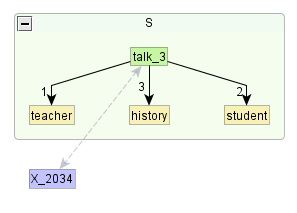
\includegraphics[width=0.4\textwidth, trim = {0cm 0cm 0cm 0cm},clip]{ch6/figs/root.png}
	\caption{Création de la racine à partir du n\oe{}ud dominant}
	\label{deroulement0}
\end{figure}


\subsection{Sélection du patron de régime dans le lexicon}
Ensuite, une fois que le n\oe{}ud dominant est lexicalisé, la règle \emph{actant\_gp\_selection} est déclenchée. Celle-ci permet à GenDR de récupérer les traits encodés pour chaque attribut \texttt{gp} d'une classe verbale. À l'intérieur de \texttt{gp}, il y a les traits \texttt{id} et \texttt{dia} qui sont donc récupérés par la règle et apposé sur la racine lexicalisée. Pour un input, le système génère autant de racine qu'il y a de GP, mais seuls ceux qui respectent les contraintes génèreront réellement des arbres, les autres seront incomplets.

\begin{figure}[htb]
	\centering
	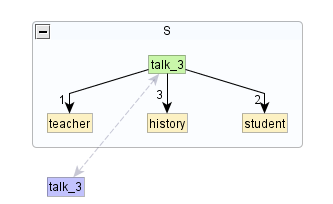
\includegraphics[width=0.4\textwidth, trim = {0cm 0cm 0cm 0cm},clip]{ch6/figs/selectiongp.png}
	\caption{Application de la règle actant\_gp\_selection}
	\label{deroulement1}
\end{figure}

\subsection{Application de la règle actancielle: \emph{actant\_gp\_ijk}}
À l'étape précédente, le n\oe{}ud \lex{talk\_3} était enrichi des traits \texttt{id} et \texttt{dia} qui sont essentiels à l'application des règles actancielles. La règle \emph{actant\_gp\_ijk} est sélectionnée lorsque la diathèse précise qu'il y a trois actants sémantiques: \lstinline|gp = { id=NP_V_PP_about_topic_PP_to_co_agent dia=132 }|. De plus, pour que l'arborisation se fasse correctement, il faut que les actants sémantiques se trouvant dans la diahtèse (\texttt{dia=132}) se retrouve dans la structure sémantique donnée. Sinon, l'application de la règle échoue. Pour l'input donné, la règle \emph{actant\_gp\_ijk} peut aussi générer un arbre à partir des \acp{GP} suivants: \texttt{id=NP\_V\_PP\_to\_co\_agent\_PP\_about\_topic}, \texttt{NP\_V\_PP\_with\_co\_agent\_PP\_about\_topic}, \texttt{NP\_V\_PP\_about\_topic\_PP\_with\_co\_agent} puisque leurs diathèses comportent les trois mêmes actants sémantiques de l'input.

Il existe ainsi jusqu'à six versions de cette règle actancielle, ce qui permet à un prédicat de sélectionner jusqu'à six actants sémantiques. Le maximum que nous avons dans ce dictionnaire est quatre actants sémantiques, mais nous voulions tenir compte de toutes les possibilités. Ce mécanisme est donc nouveau puisque dans l'ancienne version de GenDR, le système analysait chaque liaison actancielle individuellement, puis la faisait correspondre à une relation syntaxique. Cela se traduisait par la création d'un arc entre la racine et un n\oe{}ud vide qui se faisait imposer des contraintes par son gouverneur (la racine dans ce cas). La version actuelle de GenDR ne fonctionne plus ainsi, maintenant, le gp sélectionné déclenche une règle actancille en fonction du nombre d'actant compris dans sa diathèse, puis on crée des arcs en partance du gouverneur vers trois n\oe{}uds vides non-contraints.

\begin{figure}[htb]
	\centering
	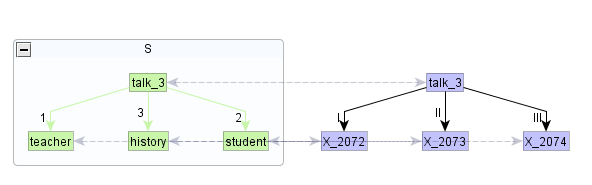
\includegraphics[width=1\textwidth, trim = {0cm 0cm 0cm 0cm},clip]{ch6/figs/actant_gp_ijk.png}
	\caption{Application d'une règle actancielle: actant\_gp\_ijk}
	\label{deroulement2}
\end{figure}

\subsection{Application des contraintes sur les n\oe{}uds}
Notre avons décidé de créer une règle qui s'occupait strictement d'imposer les contraintes aux noeuds nouvellement créés par les règles actancielles. Bref, la règle récupère les restrictions sur les n\oe{}uds qui sont encodés comme propriétés syntaxiques des \acp{GP} dans le \emph{gpcon} (voir la figure~\ref{gpexemple}). La règle d'application de contraintes s'applique trois fois puisqu'il y a trois n\oe{}uds vides, qui sont maintenant contraints par tous les traits nécessaires comme la partie du discours ou la finitude (quand un verbe sélectionne un autre verbe).

\subsection{Lexicalisation des n\oe{}uds contraints}
Ensuite, on répète la phase de lexicalisation, dans ce cas, il s'agit de \emph{lex\_standard} puisque tous les sémantèmes figurent dans le \emph{semanticon} et le \emph{lexicon}. Cette règle s'applique aussi trois fois car il y a trois n\oe{}uds. Si les propriétés des lexèmes \lex{teacher}, \lex{history} ou \lex{student} ne respectaient pas les contraintes du n\oe{}ud, alors la lexicalisation aurait échoué.
\begin{figure}[htb]
	\centering
	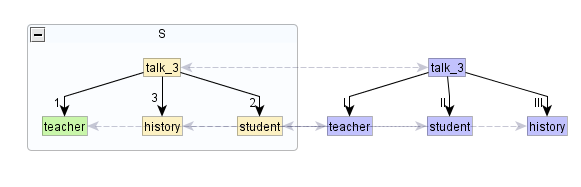
\includegraphics[width=1\textwidth, trim = {0cm 0cm 0cm 0cm},clip]{ch6/figs/lex.png}
	\caption{Applications d'une règle de lexicalisation: lex\_standard}
	\label{deroulement3}
\end{figure}

\subsection{Application de la règle \emph{actant\_gp\_selection}}
Finalement, la règle \emph{actant\_gp\_selection} s'applique encore une fois, bien que l'arbre semble réussi à cette étape. Toutefois, cette fois-ci, la règle est déclenchée trois fois par les lexèmes \lex{teacher},\lex{student} et \lex{history}. Comme toutes les catégories syntaxiques du lexique ont au moins un patron de régime, le système doit récupérer les traitss \texttt{id} et \texttt{dia} au cas où l'arborisation ne serait pas terminée. 

Comme ce sont tous des noms communs, ils héritent du ac{GP} par défaut de la classe nominale \texttt{id=NP dia=1}. Nous n'avons pas plus d'information sur les patrons de régime des noms communs compte tenu que VerbNet se spécialisait dans les verbes, mais il existe d'autres ressources parmi celles que nous avions mentionnées qui pourrait combler cette lacune. Bref, si l'un de ces lexèmes en gouvernait un autre, on aurait pu réaliser la relation qui les liait grâce à l'application systématique de cette règle pour toutes les parties du discours.

Bref, l'application de toutes ces règles à notre input(figure~\ref{input-text}) a permi son arborisation. Nous décrirons, dans la section suivante, la construction de la structure syntaxique de surface.

\subsection{Lexicalisation de surface}
La première étape est de récupérer la lexicalisation de surface des lexèmes ainsi que leur partie du discours de surface. Pour l'instant, le procédé est le même que nous avons vu au chapitre \ref{chapgendr}.

\subsection{Règles actancielles de surface}
La lexicalisation de surface déclenche ainsi les règles actancielles superficielles. Contrairement aux règles actancielles profondes qui génèrent des groupes d'arcs, ici nous reprenons la méthode traditionnelle de GenDR. En ce sens, chaque relation profonde est réalisée par l'application d'une règle actancielle de surface et puisqu'il y a 3 arcs de dépendances (I, II et III) à réaliser, il y aura trois règles actancielles de surface d'appliquer. Pour ce faire, le système récupère la valeur du trait \texttt{rel} qui encode le nom de la relation à réaliser. C'est de cette manière que la règle \emph{synt\_subj} est déclenchée, puisque le \ac{GP} de \texttt{NP\_V\_PP\_about\_topic\_PP\_to\_co\_agent} contient de la relation subjective pour son premier actant syntaxique (voir la figure~\ref{gpexemple}).

De la même manière, la règle \emph{synt\_actant\_prep} est déclenchée une première fois pour faire la correspondance entre l'arc syntaxique qui lie \lex{talk\_3} et \lex{history}. La règle récupère ainsi le code suivant: \lstinline! II={rel=oblique dpos=N prep=about}! qui signifie que l'actant syntaxique II correspond à la relation \texttt{oblique} en RSyntS. Cette relation syntaxique de surface implique la création d'un nouveau noeud en \ac{RSyntS}. Cela est du au fait que deux relations syntaxiques de ce \ac{GP} nécessite la réalisation d'une préposition pour assurer la grammaticalité de l'arbre. Conséquemment, le n\oe{}ud profond \lex{history} se scinde en deux afin que la préposition \lex{about} fasse le pont entre le verbe et l'objet indirect qu'il sélectionne. Ce phénomène est illustré par la figure~\ref{deroulement4}. Finalement, cette règle se déclenche une seconde fois pour traiter l'actant syntaxique III \lex{students}.

\subsection{Règles des déterminants}
Pour compléter l'arborisation de surface, la règle \emph{det\_def} réalise les déterminants qui doivent apparaître en syntaxe de surface qui correspondent aux attributs que nous avions encodés dans l'input de départ. Seuls \lex{teacher} et \lex{student} gouverneront des déterminants puisqu'on veut qu'ils soient défini et indéfini. La règle de déterminant pour l'anglais réalise \lex{the} lorsque le lexème est défini en surface et \lex{a} lorsque le lexème est indéfini.
\begin{figure}[htb]
	\centering
	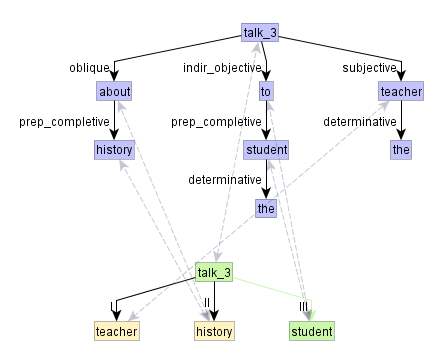
\includegraphics[width=0.5\textwidth, trim = {0cm 0cm 0cm 0cm},clip]{ch6/figs/ssynt.png}
	\caption{Applications des règles actancielles et réalisation des lexies fonctionnelles}
	\label{deroulement4}
\end{figure}
Cela met fin à notre chapitre implémentation. Nous passerons donc à la phase d'évaluation pour vérifier si notre système performe tel que nous l'avions prévu.